\subsubsection{Collection de matrices creuses de l'université de Floride}
L'application de Taggre aux problèmes des 13 nains de Berkeley n'étant pas probante, nous proposons s'appliquer sur des matrices non issues de la simulation de réservoir.
%
La collection de matrices creuses de l'université de Floride est un ensemble de matrices provenant de diverses simulations.
%
Parmi toutes ces matrices, nous en avons choisi quatre ayant des motifs différents de ceux que nous pouvons retrouver en simulation de réservoir.
%
Nous ne nous intéressons pas aux propriétés physiques de ces simulations, mais seulement aux connexions des noeuds du graphe.
%
C'est pourquoi nous allons choisir des paramètres arbitraires par rapport aux poids des tâches.
%
Ces paramètres auront une incidence sur le choix des opérateurs d'agrégations.
%
Nous testerons différents opérateurs grâce à notre simulateur.


\begin{figure}[!h]
     \begin{center}
        \subfigure[Pajek/EPA]{
          \label{fig:florida_epa}
          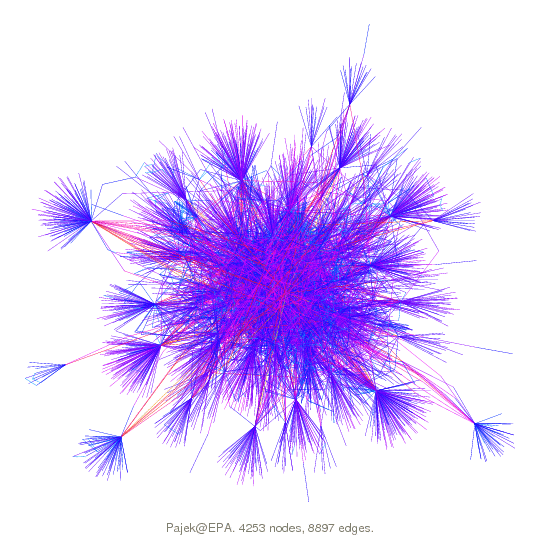
\includegraphics[width=0.45\textwidth]{florida_epa}
        } %
        ~
        \subfigure[SNAP/roadNet-PA]{
          \label{fig:florida_roadNet}
          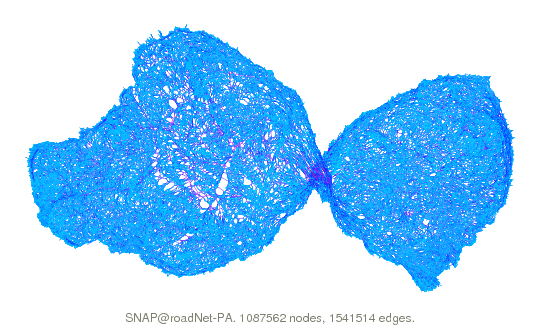
\includegraphics[width=0.45\textwidth]{florida_roadNet}
        }
        \subfigure[Gleich/wb-cs-stanford]{
          \label{fig:florida_wbcs}
          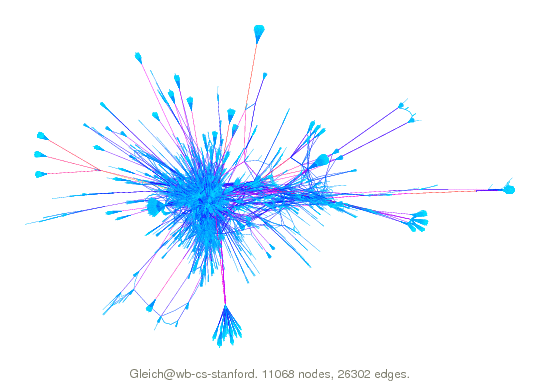
\includegraphics[width=0.45\textwidth]{florida_wbcs}
        }
        ~
        \subfigure[Williams/webbase-1M]{
          \label{fig:florida_webbase}
          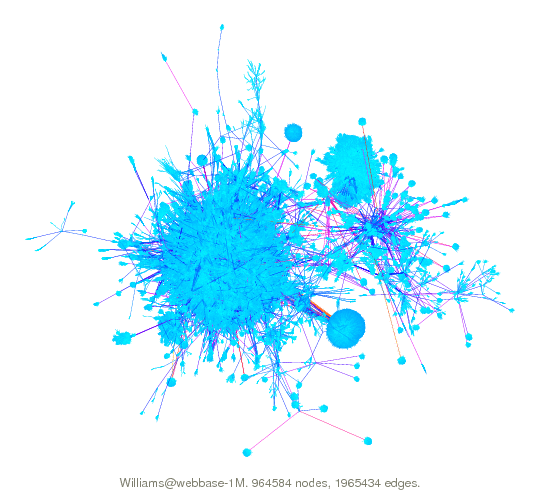
\includegraphics[width=0.45\textwidth]{florida_webbase}
        }
    \end{center}
    \caption{Représentation du graphe de connexions des quatre matrices choisies.}
    \label{fig:florida}
\end{figure}

%   (-_-)   %
\begin{center}
  \begin{tabular}{|r|c|c|c|c|}
    \hline
    Nom de la & Nombre de       & Nombre de & Paramètre des & Paramètre de\\
    matrice   & lignes/colonnes & non-zéros & effets cache  & granularité \\
    \hline
    Pajek/EPA             & 4~772     & 8~965     & 0,95 & 0,02\\
    SNAP/roadNet-PA       & 1~090~920 & 3~083~796 & 0,70 & 1\\
    Gleich/wb-cs-stanford & 9~914     & 36~854    & 0,50 & 0,001\\
    Williams/webbase-1M   & 1~000~005 & 3~105~536 & 0,98 & 0,5\\
    \hline
  \end{tabular}
  \captionof{table}{Descriptions des matrices utilisées.}
  \label{tab:florida}
\end{center}
